
\author{Anders Eiler}
\section{Design}
\subsection{What we already know}
\begin{frame}{Design}
  \begin{block}{What we already know}
  \begin{itemize}
  	\item One master-server.
  	\item One slave-server per drone. Many drones. 
  	\item One user can interact with one drone at the time.
  \end{itemize}

  \begin{figure}[htb]
    \centering
    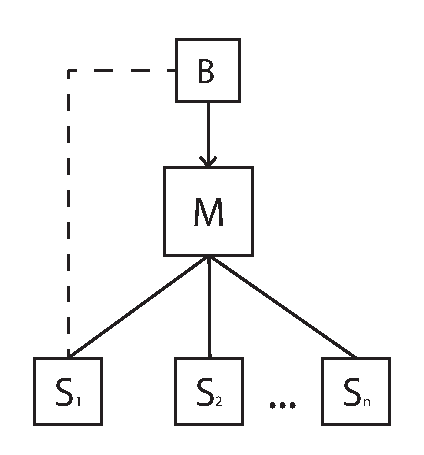
\includegraphics[width=0.35\textwidth]{gfx/slave_structure.pdf}
    \caption{LONE Structure}
  \end{figure}

  \end{block}
\end{frame}

\subsection{Privileges}
\begin{frame}{Design}{Privileges}
  \begin{block}{}
  	There are three ways of assigning privileges to many users:

  	\begin{itemize}
  		\item Each privilege to each user.
  		\item Privileges added to roles, users to roles and exceptions to users.
  		\item Lowest denominator of privileges added to roles, extra privileges added to users.
  	\end{itemize}

  \end{block}
\end{frame}

\begin{frame}{Design}{Privileges}
  \begin{block}{}
  	1 user, 7 privileges.

  	\begin{figure}[htb]
    	\centering
    	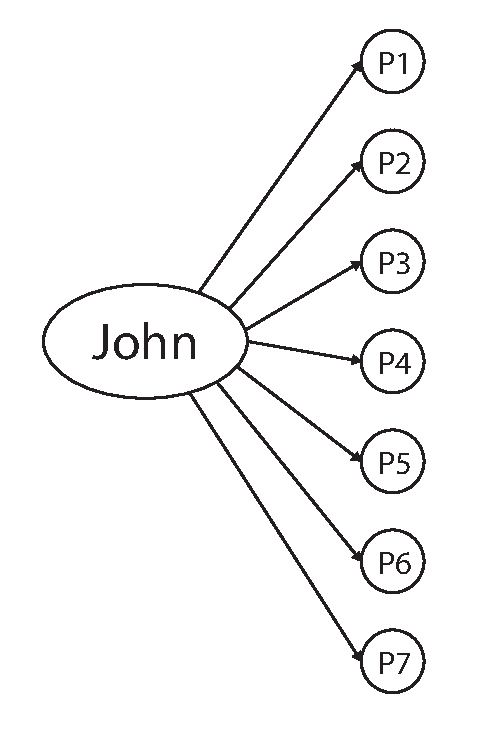
\includegraphics[width=0.35\textwidth]{images/privileges1.pdf}
  	\end{figure}
  \end{block}
\end{frame}

\begin{frame}{Design}{Privileges}
  \begin{block}{}
  	4 users, 7 privileges. 

  	\begin{figure}[htb]
    	\centering
    	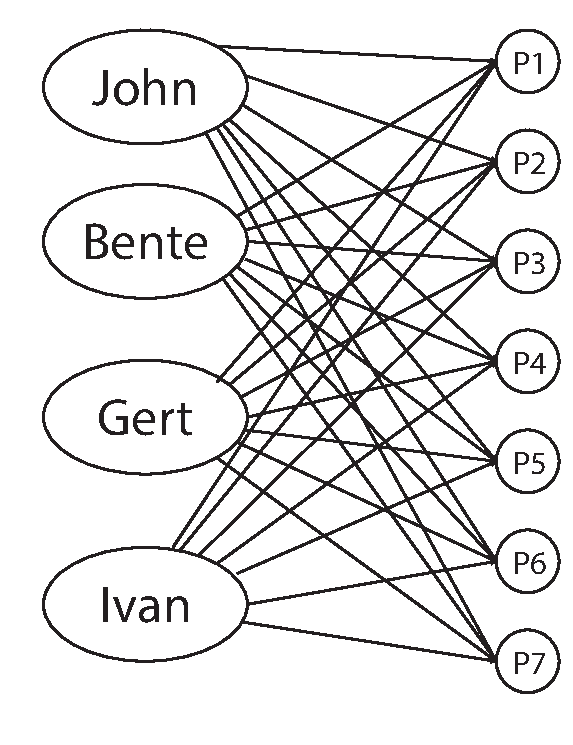
\includegraphics[width=0.35\textwidth]{images/privileges2.pdf}
  	\end{figure}
  \end{block}
\end{frame}

\begin{frame}{Design}{Privileges}
  \begin{block}{}
  	4 users, 1 role and 7 privileges

  	\begin{figure}[htb]
    	\centering
    	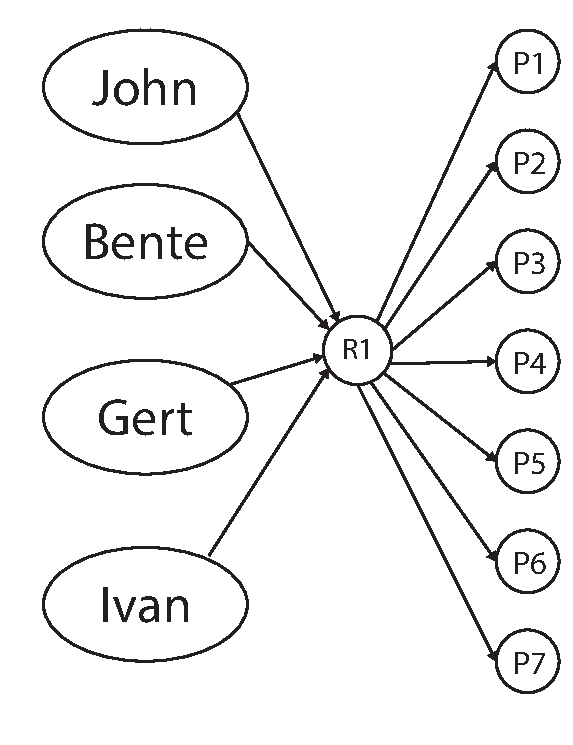
\includegraphics[width=0.35\textwidth]{images/privileges3.pdf}
  	\end{figure}
  \end{block}
\end{frame}

\begin{frame}{Design}{Privileges}
  \begin{block}{}
  	4 users, 1 role, 7 privileges (5 of those in the role, 2 directly assigned)

  	\begin{figure}[htb]
    	\centering
    	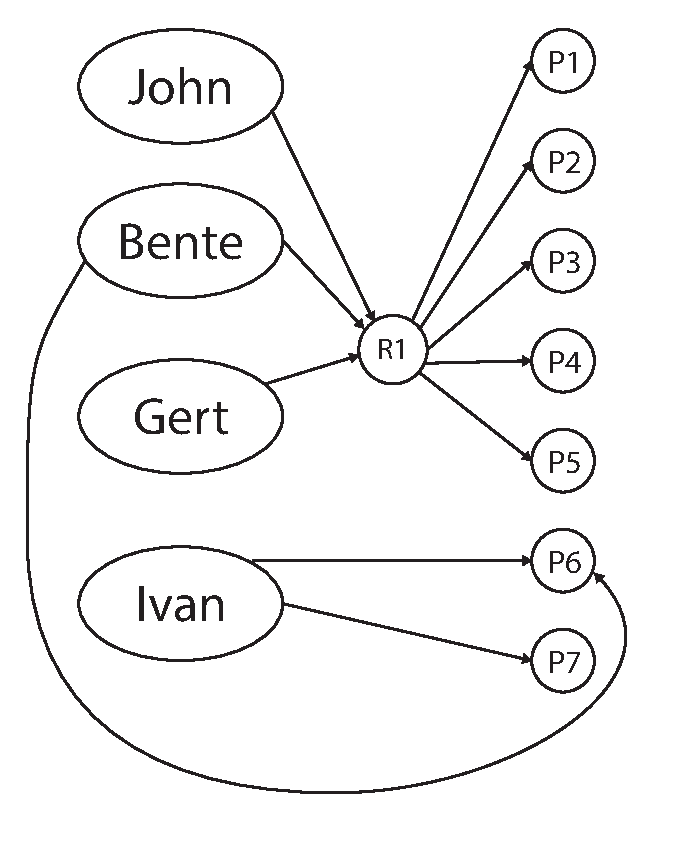
\includegraphics[width=0.35\textwidth]{images/privileges4.pdf}
  	\end{figure}
  \end{block}
\end{frame}

\begin{frame}{Design}{Privileges}
  \begin{block}{}
  	4 users, 1 role, 7 privileges (5 of those in the role, 2 directly assigned and 2 exceptions)

  	\begin{figure}[htb]
    	\centering
    	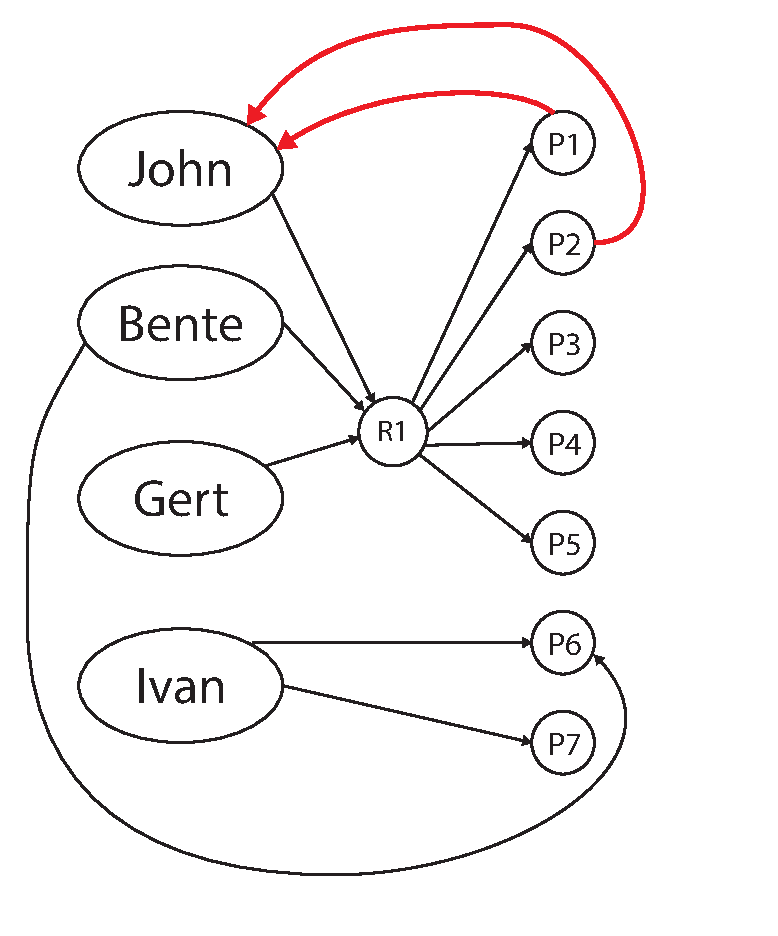
\includegraphics[width=0.35\textwidth]{images/privileges5.pdf}
  	\end{figure}
  \end{block}
\end{frame}



\subsection{Drones vs. Slaves}
\begin{frame}{Design}{Drones vs. Slaves}
  \begin{block}{How many slaves per drone, or drones per slave?}
	The current design uses one slave per drone. Is this the right design?

	Potential issues:
	\begin{itemize}
		\item Hardware overflow -- too much hardware on systems with low load.
		\item Too little hardware on systems with high load.
	\end{itemize}

	Solution?
  \end{block}
\end{frame}



\subsection{Rails Sessions}
\begin{frame}{Design}{Rails Sessions - User Authentication}
  \begin{block}{Who is that user?}
  	How do you tell users apart? We use unique identifiers, passwords and sessions. \\

  	Ruby on Rails provides a lot of tools to enhance the security when using sessions such as: \\
  	\begin{itemize}
  		\item Session ID
  		\item Protection against Session Hijacking
  		%\item Safe Session storage
  	\end{itemize}

  	Provides security measures against identity theft in the system.
  \end{block}
\end{frame}

\begin{frame}{Design}{Rails Sessions - User Authentication}
  \begin{block}{How does that relate to streaming?}
  	\begin{itemize}
  		\item Session Keys
  		\item User Authentication
  	\end{itemize}
  \end{block}
\end{frame}


%\subsection{Design outlines}
%\begin{frame}{Design outlines and decisions}{Design}
%  \begin{block}{Maintainability}
%  	\begin{itemize}
%  		\item Easy to administrate the system.
%  		\item Easy to maintain the code.
%  	\end{itemize}
%  \end{block}
%
%  \begin{block}{Scalability}
%  	\begin{itemize}
%  		\item Addition of new slaves, users and privileges.
%  		\item Addition of new types of equipment.
%  	\end{itemize}
%  \end{block}
%\end{frame}

